\documentclass{article}

\usepackage[backend=biber, style=authoryear-icomp]{biblatex}
\addbibresource{bib.bib}
%\usepackage[T2A]{fontenc}
%\usepackage[english,ukrainian]{babel}
\usepackage{fontspec}
\setmainfont{Nimbus Roman}
\usepackage{graphicx}
\usepackage[a4paper,margin=0.5in]{geometry}
\begin{document}

\pagestyle{empty}
\begin{center}

	{\fontsize{14}{24}\selectfont МІНІСТЕРСТВО ОСВІТИ І НАУКИ УКРАЇНИ

	НАЦІОНАЛЬНИЙ УНІВЕРСИТЕТ «ЛЬВІВСЬКА ПОЛІТЕХНІКА»

	Інститут комп'ютерних наук та інформаційних технологій

	}

	\vspace{90.4pt} %120.4+16.1
	\begin{figure}[h]
		\centering
		
\includegraphics[width=6.5cm,keepaspectratio]{../../lpnu.png}
	\end{figure}

	{\fontsize{18}{29}\selectfont{Звіт}

	{до практичної роботи № 2}

	{З дисципліни}

	{``Дискретна математика''}

	{на тему:}

	{``Основні операції над графами. Знаходження  мінімального кістякового дерева
за алгоритмами Пріма та Крускала''}

	}
\end{center}

\vspace{12.1pt} %30.1pt
	{\fontsize{14}{22.4}\selectfont
\begin{flushright}
	\textit{Виконав:}

	\textit{студент групи ПП-14}

	\textit{Мілюхін Олександр}

	\textit{Прийняла:}

	\textit{Ребот Д. П.}
\end{flushright}
\vspace{37.4pt} %100.4
\begin{center}
\textit{Львів-2022}
\vspace{37.4pt} %100.4
\end{center}
	}
%{\fontsize{18}{20.7}\selectfont \textbf{Лабораторна робота №1}}
{\fontsize{14}{16.1}\selectfont
\textbf{Мета:}
освоїти основні операції над графами. Навчитися знаходити
мінімальне остове дерево за алгоритмами Пріма та Крускала.

\vspace{16pt}
\centering \textbf{Варіант 12}
\section{Виконати операції над графами:}
\begin{figure}[h]
	\centering
	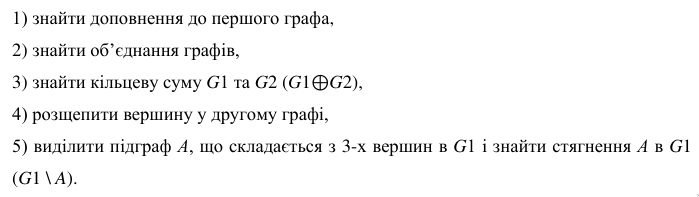
\includegraphics[width=17cm]{1.png}
	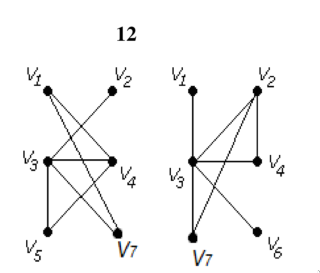
\includegraphics[width=5cm]{2.png}
\end{figure}
\section{Знайти таблицю суміжності графа:}
\begin{figure}[h]
	\centering
	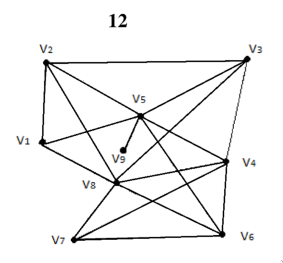
\includegraphics[width=5cm]{3.png}
\end{figure}
\section{Знайти двома методами (Пріма і Крускала) мінімальне кістякове дерево}
\begin{figure}[h]
	\centering
	
\includegraphics[width=8cm]{4.png}
\end{figure}
\begin{figure}[h]
	\centering
	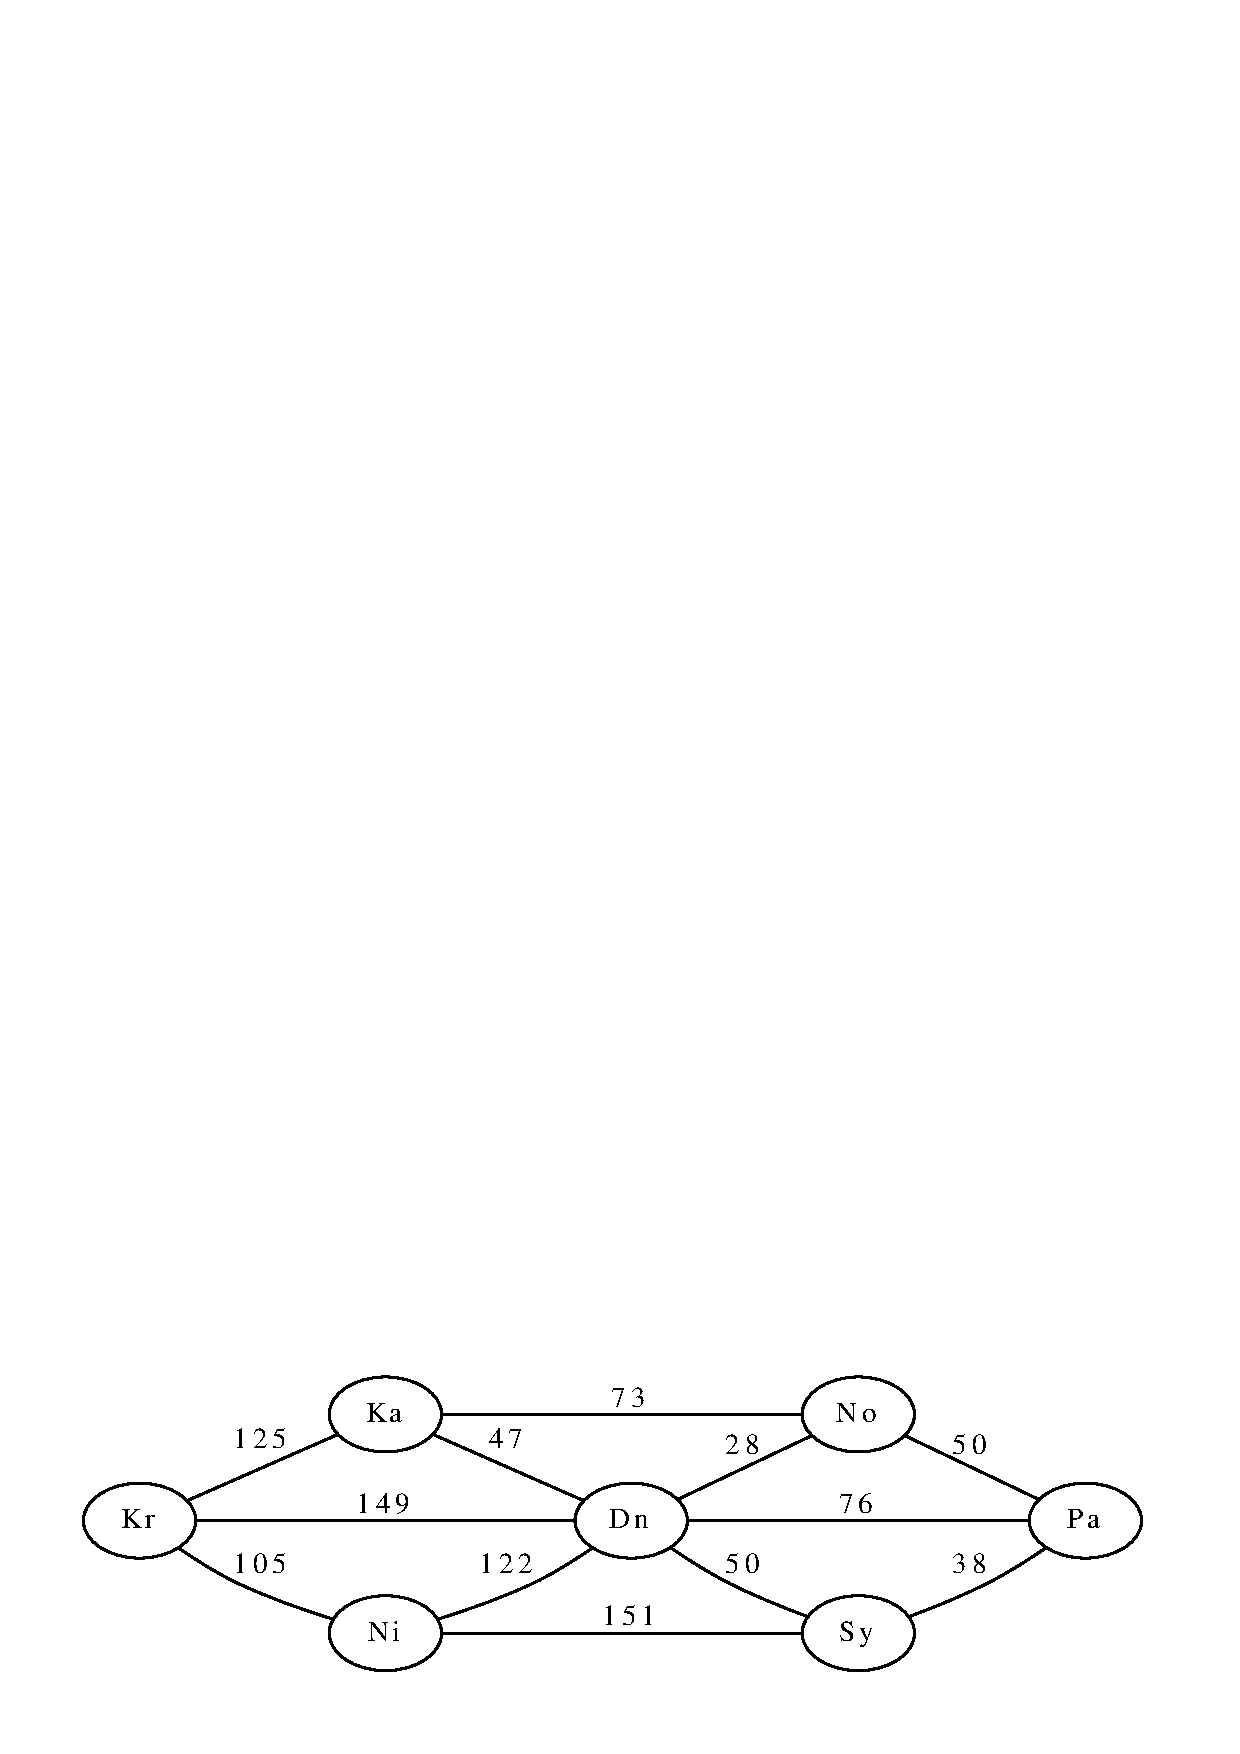
\includegraphics[width=15cm]{graph.jpg}
\end{figure}

\newpage

\textbf{Висновок:}
виконуючи цю практичну роботу, я зрозумів основні операції над графами та навчився знаходити мінімальне кістякове дерево за алгоритмами Пріма та Крускала.
}

\end{document}
